 \pstart 
 [109 r\textsuperscript{o}] \textso{Experim. V.}
  \edtext{\edlabel{poss109r2}Hinc praxis nova sequitur parandi Baroscopium}{\lemma{posse.}\xxref{poss109r1}{poss109r2}\Afootnote{ \textit{ (1) }\ \textso{Experim. V.} Construi possunt duo   \textbar\ imo plura \textit{ erg.}\ \textbar\  Baroscopia\protect\index{Sachverzeichnis}{baroscopium|textit} in eodem Tubo continuo, alterum super alterum libere pendens, non nisi aere divisa, quae tamen accedere ad se invicem non possint. \textit{ (2) }\ \textso{Experim. V.} Hinc praxis   \textbar\ nova \textit{ erg.}\ \textbar\  sequitur parandi Baroscopium \textit{ L}}}   %\begin{wrapfigure}{l}{0.1\textwidth}                    
%                                      %\caption{Bildbeschreibung}
    %                    \end{wrapfigure}
                        %@ @ @ Dies ist eine Abstandszeile - fuer den Fall, dass mehrere figures hintereinander kommen, ohne dass dazwischen laengerer Text steht. Dies kann zu einer Fahlermeldung fuehren. @ @ @ \\
                \edtext{ad usum percommodum}{\lemma{}\Afootnote{ad usum percommodum \textit{ erg.} \textit{ L}}} aeris \edtext{externi}{\lemma{}\Afootnote{externi \textit{ erg.} \textit{ L}}} mutationes indicans \edtext{aeque ut commune,}{\lemma{}\Afootnote{aeque ut commune, \textit{ erg.} \textit{ L}}}\footnote{\textit{In der rechten Spalte:} Divisio Baroscopii exacta. Attollere[.] Expurgatio aeris per Mercurii descensum.}%
%Afootnote zu footnote
 \edtext{}{\lemma{}\linenum{|19|||19|}\Afootnote{\textit{ (1) } Pondus \textit{ (2) } Divisio \textit{ L}}} 
Mercurio\protect\index{Sachverzeichnis}{mercurius} altitudinis et Tubo longitudinis quantulaecunque, \edtext{imo corpore alio exacte adaptato solido liquidove quocunque}{\lemma{}\Afootnote{imo [...] quocunque  \textit{ erg.} \textit{ L}}} dummodo altitudo Tubi sit \edtext{aliquot}{\lemma{sit}\Afootnote{ \textit{ (1) }\ tribus \textit{ (2) }\ aliquot \textit{ L}}} circiter pollicibus major altitudine Mercurii\protect\index{Sachverzeichnis}{mercurius}, quia scilicet variatio altitudinis Baroscopii\protect\index{Sachverzeichnis}{baroscopium} est aliquot pollicum inter 27. \edtext{scilicet}{\lemma{}\Afootnote{scilicet \textit{ erg.} \textit{ L}}} et 30. circiter. Id ita fiet: esto Mercurius\protect\index{Sachverzeichnis}{mercurius} altitudinis quantulaecunque \textit{ab}  %\begin{wrapfigure}{l}{0.1\textwidth}   
                        %\caption{Bildbeschreibung}
                      %  \end{wrapfigure}
                        %@ @ @ Dies ist eine Abstandszeile - fuer den Fall, dass mehrere figures hintereinander kommen, ohne dass dazwischen laengerer Text steht. Dies kann zu einer Fahlermeldung fuehren. @ @ @ \\
                         %\begin{wrapfigure}{l}{0.1\textwidth} 
                         %
\includegraphics[width=0.1\textwidth]{images/37_3_109r2}
                      %  \end{wrapfigure}
                         locatus in medio Tubi \textit{cd} clausi in summo \textit{c} et infra in \textit{d} aperti. Aer \edtext{internus}{\lemma{}\Afootnote{internus \textit{ erg.} \textit{ L}}} intra Mercurium\protect\index{Sachverzeichnis}{mercurius} et Tubi summitatem sit consistentiae ordinariae \edtext{sine tensione et compressione}{\lemma{ordinariae}\Afootnote{ \textit{ (1) }\ , qualis est \textit{ (2) }\ sine tensione et compressione \textit{ L}}} quod fiet si \edtext{tempore Mercurii}{\lemma{si}\Afootnote{ \textit{ (1) }\ Mercurio \textit{ (2) }\ tempore Mercurii \textit{ L}}} introducti extremum \textit{c} sit apertum postea claudatur. Ita aer \edtext{\textit{ca}}{\lemma{}\Afootnote{\textit{ca} \textit{ erg.} \textit{ L}}} non erit tensus, quia pondus\protect\index{Sachverzeichnis}{pondus} \textit{ab} non descendit est enim 27 pollicibus minus, per dicta Exp. praeced. Hinc pondus\protect\index{Sachverzeichnis}{pondus} seu pressio aeris\protect\index{Sachverzeichnis}{pressio!aeris} externi nec demittet Mercurium\protect\index{Sachverzeichnis}{mercurius} \textit{ab} quia is non satis fortis est ad eam pressionem superandam, nec sursum pellet versus \textit{c} quia aer \textit{ca} est ordinarius, et allevato Mercurio\protect\index{Sachverzeichnis}{mercurius} \textit{ab} ultra statum ordinarium esset comprimendus cum tamen atmosphaerae\protect\index{Sachverzeichnis}{atmosphaera} pressio in aerem\protect\index{Sachverzeichnis}{pressio!aeris} ordinarium nihil possit, nisi quatenus ejus gravitas\protect\index{Sachverzeichnis}{gravitas}\edtext{}{\lemma{}\Afootnote{gravitas  \textbar\ nunc \textit{ gestr.}\ \textbar\ augetur. \textit{ L}}} augetur. Nam si minuitur, tantum abest ut agat in aerem ordinarium, ut aer ordinarium, agat in externum, eumque repellat. Ergo Mercurius\protect\index{Sachverzeichnis}{mercurius} \textit{ab} attolletur tantum, \edtext{quando}{\lemma{tantum,}\Afootnote{ \textit{ (1) }\ quantum \textit{ (2) }\ quando \textit{ L}}} pressio aeris\protect\index{Sachverzeichnis}{pressio!aeris} externi augebitur, et descendet, quando pressio aeris\protect\index{Sachverzeichnis}{pressio!aeris} externi minuetur. Hoc Baroscopio\protect\index{Sachverzeichnis}{baroscopium} nihil est commodius, \edtext{nihil simplicius}{\lemma{}\Afootnote{nihil simplicius \textit{ erg.} \textit{ L}}} cum sufficiat magnitudo quanta hic expressa est, \edlabel{qual109r1}qualis  portabilis est manui\footnote{\textit{Über} manui: imo} \edtext{et huc illuc ferri potest sine ullo effluxionis metu\edlabel{qual109r2}}{\lemma{qualis}\xxref{qual109r1}{qual109r2}\Afootnote{ \textit{ (1) }\ manui includi potest \textit{ (2) }\ portabilis [...] metu \textit{ L}}}. \edtext{Potest}{\lemma{metu.}\Afootnote{ \textit{ (1) }\ Cumque \textit{ (2) }\ Adde quod \textit{ (3) }\ Potest \textit{ L}}} loco Mercurii\protect\index{Sachverzeichnis}{mercurius} liquor\protect\index{Sachverzeichnis}{liquor} alius quilibet adhiberi, neque enim pondus\protect\index{Sachverzeichnis}{pondus} quicquam ad rem pertinet. Quia non inter \textit{ab} et aerem externum, sed inter aerem externum \textit{bd} et ultra, internumque \textit{ac} aequilibrium\protect\index{Sachverzeichnis}{aequilibrium} est, pro cujus variationibus ab \edtext{externi statu}{\lemma{ab}\Afootnote{ \textit{ (1) }\ aeris statu \textit{ (2) }\ externi statu \textit{ L}}} pendentibus, \textit{ab} in medio positum huc illuc fluctuat. Ergo adhiberi potest etiam corpus solidum tubo exacte aptatum. \edtext{Sed labor a solido hic major duratio minor, commoditas nulla. Satius ergo liquidum retinetur. Huic}{\lemma{aptatum.}\Afootnote{ \textit{ (1) }\ Sed \textit{ (2) }\ Huic solido \textit{ab} insistere aut huic \textit{ (3) }\ Sed labor   \textbar\ a solido \textit{ erg.}~\textbar\  hic major   \textbar\ duratio minor \textit{ erg.}\ \textbar\ commoditas, [...] Huic \textit{ L}}} liquido \textit{ab} innatare potest virunculus digito \edtext{numeros in Tubo per scalam descriptos}{\lemma{digito}\Afootnote{ \textit{ (1) }\ notas \textit{ (2) }\ numeros in Tubo   \textbar\ per scalam \textit{ erg.}\ \textbar\  descriptos \textit{ L}}} designans.
                         \pend  
% Zeitz auskommentiert                        \begin{center}
% 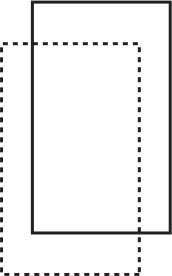
\includegraphics[width=0.09\textwidth]{images/37_3_109r1}     \hspace{2cm}          
%                
\includegraphics[width=0.09\textwidth]{images/37_3_109r2}\hspace{2cm}
%                
\includegraphics[width=0.09\textwidth]{images/37_3_109r3}\\\textit{[Fig. 5, gestr.]}  \hspace{1cm}\textit{[Fig. 6, gestr.]}\hspace{1.5cm}\textit{[Fig. 7]}\rule[0cm]{0.5cm}{0cm}
%                \end{center}
               